%!TEX root = ../main.tex

\section{Boundary Integral Formulation}
\label{sec:BoundaryIntegralFormulation}

We consider a bounded open domain $\Omega\subseteq\mathbb{R}^3$ with Lipschitz boundary $\Gamma=\partial\Omega$, and we want to solve potential problems described by the Laplace equation
\begin{equation}
\label{eq:poisson-eq}
\Delta \phi=0\qquad \text{ in }\Omega.
\end{equation}

We couple Eq.~\eqref{eq:poisson-eq} with the following boundary conditions:
\begin{subequations}
\label{eq:BCs}
\begin{align}
\label{eq:Dirichlet}
\phi=f_D &\qquad \text{ on }\Gamma_D, \\
\label{eq:Neumann} 
\frac{\partial\phi}{\partial n}=f_N &\qquad \text{ on }\Gamma_N, 
\end{align}
\end{subequations}

where $\frac{\partial \phi}{\partial n}=\nabla \phi\cdot \mathbf{n}$, $\Gamma_D\cup\Gamma_N=\Gamma$, $\Gamma_D\cap\Gamma_N=\varnothing$, and $\Gamma_D\neq\varnothing$.

\subsection{Laplace Equation in Distributional Form}
\label{sub:lapDistrib}%

Before dealing with Eq.~\eqref{eq:poisson-eq}, let us consider the following equation:
\begin{equation}
\label{eq:fundamental-eq}
-\Delta \phi(\mathbf{y})=\delta_\mathbf{x}\qquad\forall\,\mathbf{y}\in\mathbb{R}^3.
\end{equation}

This is known as the Poisson equation in the whole space. Here, $\phi(\mathbf{y})$ represents the potential produced at a point $\mathbf{y}$ in the domain $\Omega$ generated by a unit point source placed at point $\mathbf{x}$, i.e., the Dirac Delta function $\delta_\mathbf{x}$. A solution of Eq.~\eqref{eq:fundamental-eq} is called the fundamental solution of the laplacian, and it can be determined as follows.

We write Eq.~\eqref{eq:fundamental-eq} in polar coordinates with origin at $\mathbf{x}$. Since this solution is axisymmetric with respect to the source, it is independent of the polar angle $\theta$, thus the three-dimensional laplacian is
\begin{equation*}
\Delta \phi = \phi_{rr} + \frac{2}{r}\ \phi_r,
\end{equation*}

where $r=\left| \mathbf{x}-\mathbf{y} \right|$ is the Euclidean distance between $\mathbf{x}$ and $\mathbf{y}$. The right-hand side vanishes at all points of the plane, except at the origin $r=0$ (or $\mathbf{y}=\mathbf{x}$), where it has infinite value. Then Eq.~\eqref{eq:fundamental-eq} is written as
\begin{equation*}
\phi_{rr} + \frac{2}{r}\ \phi_r = 0 \qquad \forall\, r>0.
\end{equation*}

The change of variables $\phi_r=v$ gives us 
\begin{equation*}
\begin{gathered}
v' + \frac{2}{r}\ v = 0 \quad \leadsto \quad \int \frac{v'}{v}= \int -\frac{2}{r}  \\ \leadsto \quad \log(v) =-2\log(r)+c \quad \leadsto \quad v=\frac{c}{r^2}  ,  
\end{gathered}
\end{equation*}

then 
\begin{equation*}
\phi=\int \frac{c}{r^2} = \frac{c_1}{r} +c_2.
\end{equation*}

Since we want a particular solution we may set $c_2=0$, and to determine $c_1$ we perform an integration by parts on Eq.~\eqref{eq:fundamental-eq} over a ficticious unit circular domain $\Omega$:
\begin{equation*}
\int_\Omega -\Delta \phi\ \varphi \ \mathrm{d}\Omega = -\int_{\partial\Omega}\frac{\partial \phi}{\partial n}\ \varphi \ \mathrm{d}S+\int_\Omega \nabla \phi \cdot \nabla \varphi \ \mathrm{d}\Omega
\end{equation*}

which, for $\varphi\equiv 1$, reads
\begin{equation*}
\int_\Omega \delta_\mathbf{x}\ \mathrm{d}\Omega = \int_{\partial\Omega}\frac{\partial \phi}{\partial n} \ \mathrm{d}S.
\end{equation*}

Due to the axisymmetric nature of the problem
\begin{equation*}
\frac{\partial \phi}{\partial n}=\frac{\partial \phi}{\partial r} = \frac{c_1}{r^2}
\end{equation*}
thus, after using the definition of Delta function and performing an integration in radial coordinates, we are left with
\begin{equation*}
1=4\pi \int_0^1 \rho^2\ v(\rho) \ \mathrm{d}\rho = 4\pi \int_0^1 \rho^2\ \frac{c_1}{\rho^2} \ \mathrm{d}\rho =4\pi c_1.
\end{equation*}

We discovered $c_1=\frac{1}{4\pi}$, hence, the fundamental solution becomes $\phi=\frac{1}{4\pi r}$, which is also known in the literature as the free space Green's function:
\begin{equation}
\label{eq:green-fun}
G(\mathbf{x},\mathbf{y})=\frac{1}{4\pi \left| \mathbf{x}-\mathbf{y} \right|}\qquad \forall\,\mathbf{y}\in\mathbb{R}^3.
\end{equation}

One can easily prove (see for example \ref{Evans}) that this expression is the solution of $-\Delta G(\mathbf{x},\cdot)=\delta_\mathbf{x}$ in $\mathcal{D}'(\mathbb{R}^3)$, i.e., in the distributional sense. 

\subsection{BEM for the Laplace Equation}
\label{sub:bem_for_the_laplace_equation}

Here we derive the solution of the Laplace equation~\eqref{eq:poisson-eq} with mixed boundary conditions~\eqref{eq:BCs}. 

We can multiply the Laplace equation by an arbitrary test function $\varphi$ and integrate by parts twice:
\begin{gather*}
0=\int_\Omega -\Delta \phi\ \varphi \ \mathrm{d}\Omega = - \int_{\Gamma} \frac{\partial \phi}{\partial n}\ \varphi \ \mathrm{d}S + \int_\Omega \nabla \phi\ \nabla \varphi\ \mathrm{d}\Omega \\ 
= - \int_{\Gamma} \frac{\partial \phi}{\partial n}\ \varphi \ \mathrm{d}S + \int_{\Gamma} \frac{\partial \varphi}{\partial n}\ \phi \ \mathrm{d}S - \int_\Omega \Delta \varphi\ \phi\ \mathrm{d}\Omega
\end{gather*}

(one could directly apply the Green's second identity). Choosing $\varphi\equiv G$, the free space Green's function defined in Eq.~\eqref{eq:green-fun}, Laplace Eq.~\eqref{eq:poisson-eq} becomes
\begin{equation*}
\int_\Omega -\Delta G\ \phi(\mathbf{y})\ \mathrm{d}\Omega(\mathbf{y}) = \int_{\Gamma} \left[ \frac{\partial \phi}{\partial n}(\mathbf{y})\ G - \frac{\partial G}{\partial n}\ \phi(\mathbf{y}) \right]\!\! \ \mathrm{d}S(\mathbf{y}).
\end{equation*}

Since we know that $-\Delta G(\mathbf{x},\mathbf{y})=\delta_\mathbf{x}$,
\begin{equation*}
\int_\Omega \delta_\mathbf{x}\ \phi(\mathbf{y})\ \mathrm{d}\Omega(\mathbf{y}) = \int_{\Gamma} \left[ \frac{\partial \phi}{\partial n}(\mathbf{y})\ G- \frac{\partial G}{\partial n}\ \phi(\mathbf{y}) \right]\!\! \ \mathrm{d}S(\mathbf{y})
\end{equation*}

hence, by the definition of Dirac Delta, we are left with
\begin{equation}
\label{eq:integral-rep}
\phi(\mathbf{x}) = \int_{\Gamma} \left[ \frac{\partial \phi}{\partial n}(\mathbf{y})\ G(\mathbf{x},\mathbf{y}) - \frac{\partial G}{\partial n}(\mathbf{x},\mathbf{y})\ \phi(\mathbf{y}) \right]\!\! \ \mathrm{d}S(\mathbf{y})
\end{equation}

$\forall\, \mathbf{x} \in\Omega$. This expression is the integral representation of the solution for the Laplace equation at any point $\mathbf{x}$ inside the domain $\Omega$ in terms of the boundary values of $\phi$ and its normal derivative ${\partial \phi}/{\partial n}$. It is apparent from the boundary conditions~\eqref{eq:Dirichlet} and~\eqref{eq:Neumann}, that only one of the quantities $\phi$ or $\partial\phi/\partial n$ is prescribed at a point $\mathbf{y}$ on the boundary.  Consequently, it is not yet possible to determine the solution from the integral representation~\eqref{eq:integral-rep}. Therefore, we let $\mathbf{x}$ lie on the boundary $\Gamma$: we notiche that the kernels $G(\mathbf{x},\mathbf{y})$ and $\frac{\partial G}{\partial n}(\mathbf{x},\mathbf{y})$ become weakly singular (but integrable) and singular respectively. Hence, considering the Cauchy Principal Value (CPV) of the $\frac{\partial G}{\partial n}$ singular integral, we can write
\begin{equation}
\label{eq:solid-angle}
\resizebox{.9\hsize}{!}{
$\alpha(\mathbf{x})\phi(\mathbf{x}) = \displaystyle\int_{\Gamma} \frac{\partial \phi}{\partial n}(\mathbf{y})\ G(\mathbf{x},\mathbf{y})\ \mathrm{d}S(\mathbf{y}) - \int_{\Gamma}^{\text{PV}} \frac{\partial G}{\partial n}(\mathbf{x},\mathbf{y})\ \phi(\mathbf{y}) \ \mathrm{d}S(\mathbf{y}),$}
\end{equation}

where the coefficient $\alpha(\mathbf{x})$ is obtained fromt the CPV evaluation of the singular integral, and it represents the fraction of solid angle (see Fig.~\ref{fig:angle}) with which the domain $\Omega$ is seen from the boundary point $\mathbf{x}$:
\begin{equation*}
\alpha(\mathbf{x})=
\begin{cases}
1 &\text{ for } \mathbf{x} \text{ inside } \Omega, \\ 
\textstyle\frac{\theta_1-\theta_2}{2\pi} &\text{ for } \mathbf{x} \text{ on the boundary } \Gamma, \\
0 &\text{ for } \mathbf{x} \text{ outside } \Omega.
\end{cases}
\end{equation*}

In particular, $\alpha=1/2$ for smooth boundary points.

\begin{figure}
  \begin{center}
    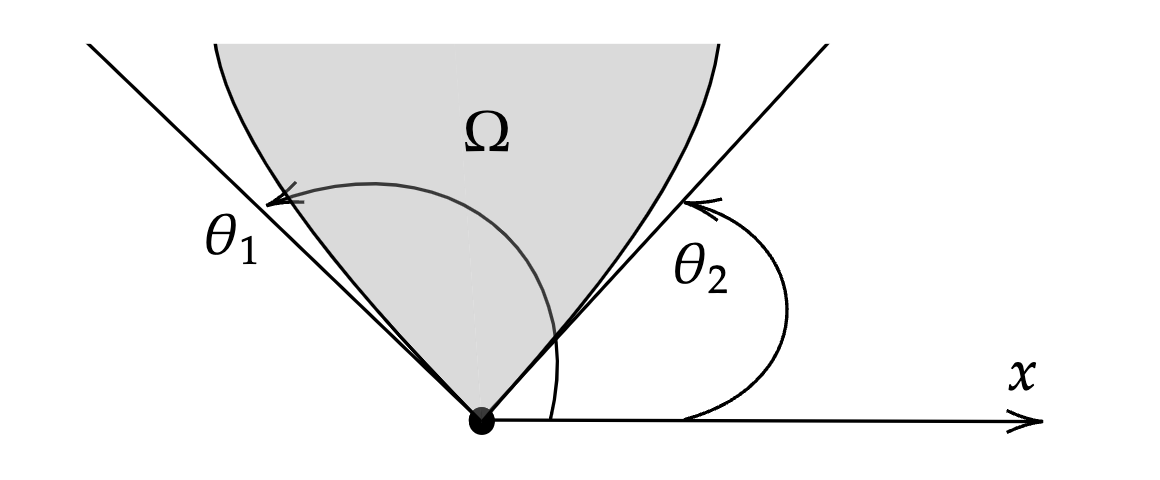
\includegraphics[width=8.4cm]{angle}    % The printed column width is 8.4 cm.
    \caption{Solid angle related to a corner point of a nonsmooth boundary.} 
    \label{fig:angle}
  \end{center}
\end{figure}

By explicitly writing the boundary conditions using the characteristic function $\chi_{_A}(\mathbf{x})$, which is one if $\mathbf{x}\in A$ and zero otherwise, we obtain
\begin{equation*}
\begin{gathered}
\resizebox{.9\hsize}{!}{
$\chi_{_{\Gamma_{\!N}}}\!(\mathbf{x})\alpha(\mathbf{x})\phi(\mathbf{x}) - \displaystyle\int_{\Gamma_{\!N}} f_{_N}(\mathbf{y})\ G(\mathbf{x},\mathbf{y})\ \mathrm{d}S(\mathbf{y}) + \int_{\Gamma_{\!N}}^{\text{PV}} \frac{\partial G}{\partial n}(\mathbf{x},\mathbf{y})\ \phi(\mathbf{y}) \ \mathrm{d}S(\mathbf{y})=$} \\
\resizebox{.9\hsize}{!}{
$= - \chi_{_{\Gamma_{\!D}}}\!(\mathbf{x})\alpha(\mathbf{x})f_{_D}(\mathbf{x}) + \displaystyle\int_{\Gamma_{\!D}} \frac{\partial\phi}{\partial n}(\mathbf{y})\ G(\mathbf{x},\mathbf{y})\ \mathrm{d}S(\mathbf{y}) - \int_{\Gamma_{\!D}}^{\text{PV}} \frac{\partial G}{\partial n}(\mathbf{x},\mathbf{y})\ f_{_D}(\mathbf{y}) \ \mathrm{d}S(\mathbf{y}).$}
\end{gathered}
\end{equation*}

Grouping all the unknowns in the left-hand side we finally deduce
\begin{equation}
\label{eq:characteristic-angle}
\begin{gathered}
\resizebox{.9\hsize}{!}{
$\chi_{_{\Gamma_{\!N}}}\!(\mathbf{x})\alpha(\mathbf{x})\phi(\mathbf{x}) - \displaystyle\int_{\Gamma_{\!D}} \frac{\partial \phi}{\partial n}(\mathbf{y})\ G(\mathbf{x},\mathbf{y})\ \mathrm{d}S(\mathbf{y}) + \int_{\Gamma_{\!N}}^{\text{PV}} \frac{\partial G}{\partial n}(\mathbf{x},\mathbf{y})\ \phi(\mathbf{y}) \ \mathrm{d}S(\mathbf{y})=$} \\
\resizebox{.9\hsize}{!}{
$= - \chi_{_{\Gamma_{\!D}}}\!(\mathbf{x})\alpha(\mathbf{x})f_{_D}(\mathbf{x}) + \displaystyle\int_{\Gamma_{\!N}} f_{_N}(\mathbf{y})\ G(\mathbf{x},\mathbf{y})\ \mathrm{d}S(\mathbf{y}) - \int_{\Gamma_{\!D}}^{\text{PV}} \frac{\partial G}{\partial n}(\mathbf{x},\mathbf{y})\ f_{_D}(\mathbf{y}) \ \mathrm{d}S(\mathbf{y}).$}
\end{gathered}
\end{equation}

Eq.~\eqref{eq:characteristic-angle} simply is the trace of Eq.~\eqref{eq:integral-rep}, namely it is the BIE with which it is possible to derive the potential where its normal derivative is known, and viceversa.








